\usepackage{graphicx}
\begin{document}
\section{PIR Sensor}
PIR (Passive Infrared Receiver) merupakan sebuah sensor berbasiskan infrared. Akan tetapi, tidak seperti sensor infrared kebanyakan yang terdiri dari IR LED 
dan fototransistor. PIR tidak memancarkan apapun seperti IR LED. Sesuai dengan namanya \"Passive\", sensor ini hanya merespon energi dari pancaran sinar 
inframerah pasif yang dimiliki oleh setiap benda yang terdeteksi olehnya. Benda yang bisa dideteksi oleh sensor ini biasanya adalah tubuh manusia.

	\subsection{Cara Kerja}
	PIR (Passive Infrared Receiver) merupakan sebuah sensor berbasiskan infrared. Akan tetapi, tidak seperti sensor infrared kebanyakan yang terdiri dari IR LED 
	dan fototransistor. PIR tidak memancarkan apapun seperti IR LED. Sesuai dengan namanya \"Passive\", sensor ini hanya merespon energi dari pancaran sinar 
	inframerah pasif yang dimiliki oleh setiap benda yang terdeteksi olehnya. Benda yang bisa dideteksi oleh sensor ini biasanya adalah tubuh manusia.

	Mengapa sensor PIR hanya bereaksi pada tubuh manusia saja? Hal ini disebabkan karena adanya IR Filter yang menyaring panjang gelombang sinar inframerah pasif. 
	IR Filter dimodul sensor PIR ini mampu menyaring panjang gelombang sinar inframerah pasif antara 8 sampai 14 mikrometer, sehingga panjang gelombang yang 
	dihasilkan dari tubuh manusia yang berkisar antara 9 sampai 10 mikrometer ini saja yang dapat dideteksi oleh sensor.

	Jadi, ketika seseorang berjalan melewati sensor, sensor akan menangkap pancaran sinar inframerah pasif yang dipancarkan oleh tubuh manusia yang memiliki suhu 
	yang berbeda dari lingkungan sehingga menyebabkan material pyroelectric bereaksi menghasilkan arus listrik karena adanya energi panas yang dibawa oleh sinar 
	inframerah pasif tersebut. Kemudian sebuah sirkuit amplifier yang ada menguatkan arus tersebut yang kemudian dibandingkan oleh comparator sehingga menghasilkan 
	output.

	Ketika manusia berada di depan sensor PIR dengan kondisi diam, maka sensor PIR akan menghitung panjang gelombang yang dihasilkan oleh tubuh manusia tersebut. 
	Panjang gelombang yang konstan ini menyebabkan energi panas yang dihasilkan dapat digambarkan hampir sama pada kondisi lingkungan disekitarnya. Ketika manusia 
	itu melakukan gerakan, maka tubuh manusia itu akan menghasilkam pancaran sinar inframerah pasif dengan panjang gelombang yang bervariasi sehingga menghasilkan 
	panas berbeda yang menyebabkan sensor merespon dengan cara menghasilkan arus pada material Pyroelectricnya dengan besaran yang berbeda beda. Karena besaran 
	yang berbeda inilah comparator menghasilkan output.

	Jadi sensor PIR tidak akan menghasilkan output apabila sensor ini dihadapkan dengan benda panas yang tidak memiliki panjang gelombang inframerah antar 8 sampai 
	14 mikrometer dan benda yang diam seperti sinar lampu yang sangat terang yang mampu menghasilkan panas, pantulan objek benda dari cermin dan suhu panas ketika 
	musim panas.

	Untuk jarak jangkau dari sensor PIR sendiri bisa disetting sesuai kebutuhan, akan tetapi jarak maksimalnya hanya +/- 10 meter dan minimal +/- 30 cm.

	\begin{figure}[ht]
		\centerline{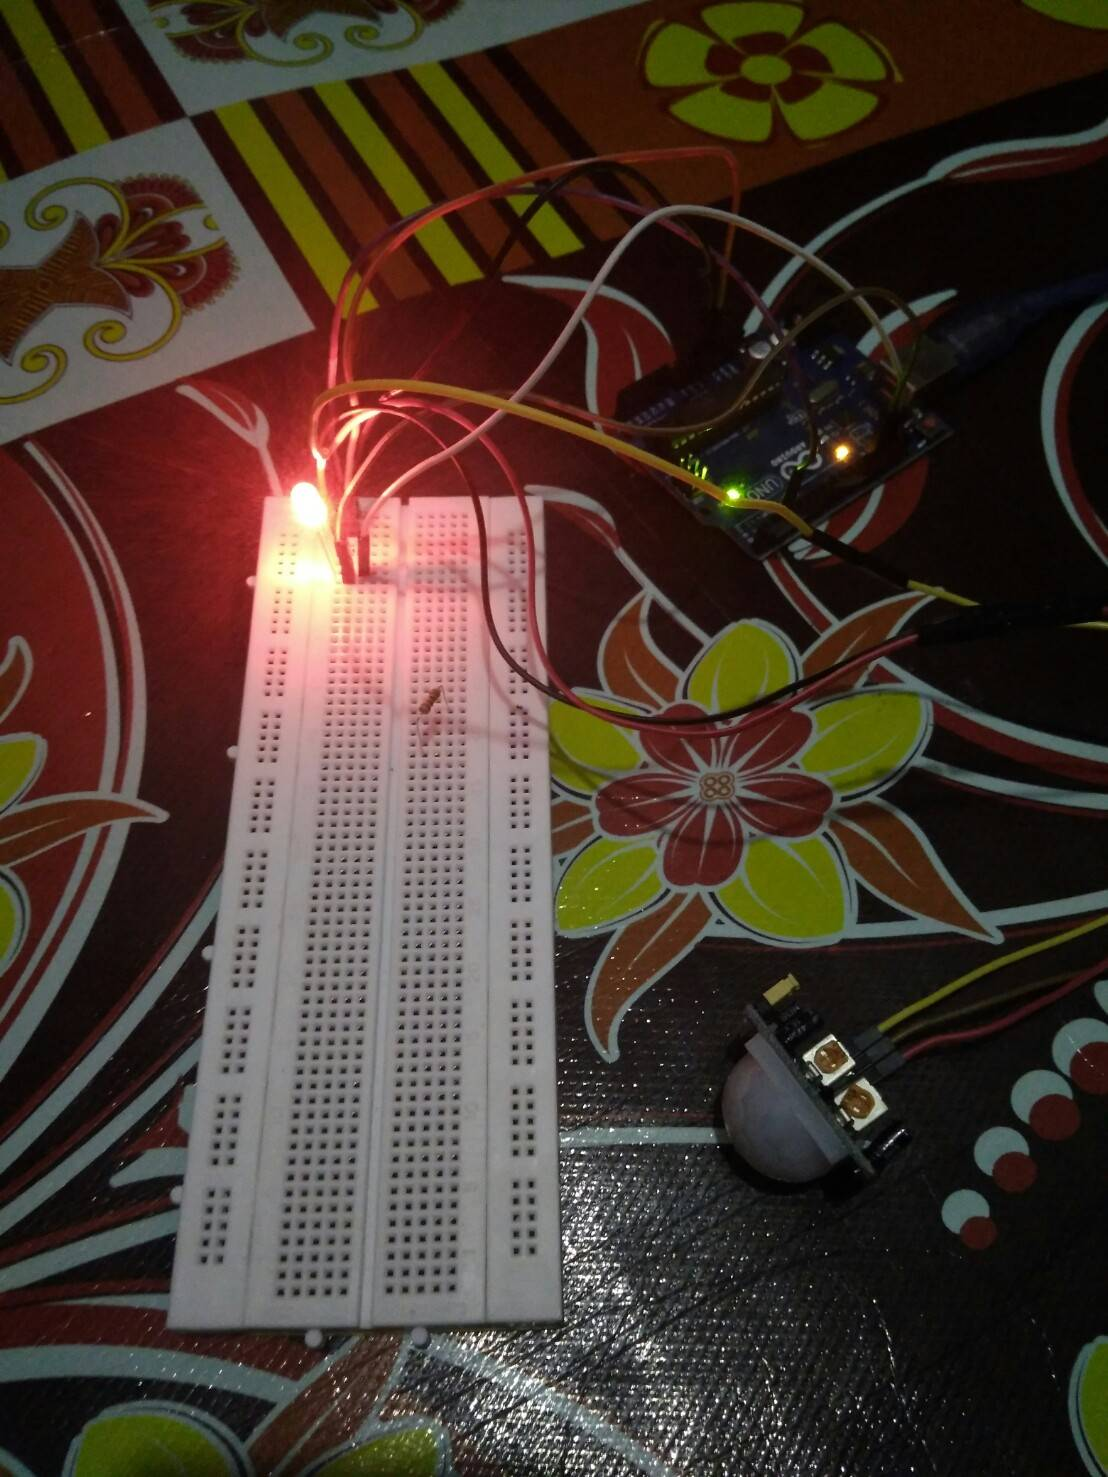
\includegraphics[width=1\textwidth]{figures/project_arduino.jpg}}
		\caption{Hasil dari PIR sensor.}
		\label{project_arduino}
	\end{figure}

	\subsection{Kodingan}
	\begingroup\makeatletter\def\@currenvir{verbatim}
		\verbatim
		int led = 13;                
		int sensor = 2;              
		int state = LOW;             
		int val = 0;                 

		void setup() {
			pinMode(led, OUTPUT);    
			pinMode(sensor, INPUT);  
			Serial.begin(9600);      
			}

		void loop(){
			val = digitalRead(sensor); 
			if (val == HIGH) {         
			  digitalWrite(led, HIGH); 
			  delay(100);               
    
				if (state == LOW) {
				  Serial.println("Motion detected!"); 
				  state = HIGH;       
				}
			} 
			else {
				digitalWrite(led, LOW);
				delay(200);             
      
				if (state == HIGH){
				  Serial.println("Motion stopped!");
				  state = LOW;
			}
		  }
		}
	\end{verbatim}

	\begin{figure}[ht]
		\centerline{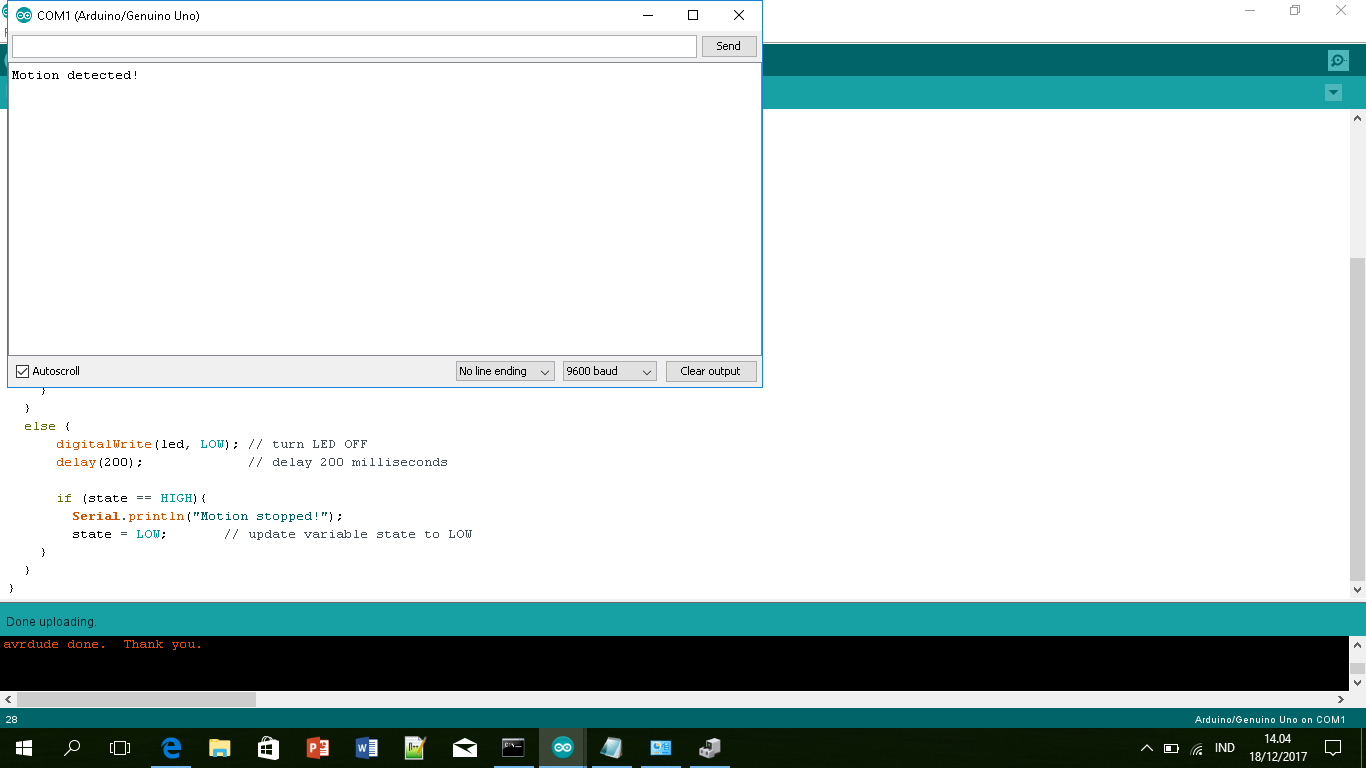
\includegraphics[width=1\textwidth]{figures/serial_monitor.PNG}}
		\caption{serial monitor.}
		\label{project_arduino}
	\end{figure}